% !TeX spellcheck = en_US
%% Beispiel-Präsentation mit LaTeX Beamer im KIT-Design
%% entsprechend den Gestaltungsrichtlinien vom 1. August 2020
%%
%% Siehe https://sdqweb.ipd.kit.edu/wiki/Dokumentvorlagen

%% Beispiel-Präsentation
\documentclass[en,16:9]{sdqbeamer} 

\usepackage{tikz}
\usetikzlibrary{positioning,calc,arrows}
\usepackage{pgf-pie}  
 
 
%% Titelbild
\titleimage{banner_2020_kit}

%% Gruppenlogo
\grouplogo{} 

%% Gruppenname
\groupname{Compilerpraktikum - Abschlusspräsentation}

% Beginn der Präsentation

\title[]{Compilerpraktikum - Abschlusspräsentation}
\subtitle{Gruppe 5} 
\author[]{Achim Kriso, Marc Huisinga, Erik Kristiansen, Philipp Schaback}

\date[10.\,2.\,2022]{10. Februar 2022}

% Literatur 
 
\usepackage[citestyle=authoryear,bibstyle=numeric,hyperref,backend=biber]{biblatex}
\addbibresource{presentation.bib}
\bibhang1em

\begin{document}

%Titelseite
\KITtitleframe

\begin{frame}{Instruction Selection - Overview}
	\begin{itemize}
		\item Macro Substitution
		\begin{itemize}
			\item Translate one IR-instruction to one or more target instructions
		\end{itemize}
		\vspace{1em}
		\item Bottom-Up Pattern Matching (BUPM)
		\begin{itemize}
			\item Apply tree patterns to IR
			\item Choose the best combination using dynamic programming
		\end{itemize}
		\vspace{1em}
		\item DAG Matching
		\begin{itemize}
			\item Apply DAG patterns to IR (greedy)
		\end{itemize}
	\end{itemize}
\end{frame}

\begin{frame}{Instruction Selection - Macro Substitution}
	\begin{columns}
		\begin{column}{0.5\textwidth}
			\begin{itemize}
				\item Generates instructions using simple rules
				\item Has very little context (can inspect inputs)
				\vspace{3em}
				\item \texttt{V3 <- mul V1 0x4}
				\item \texttt{V4 <- add V2 V3}
				\item \texttt{v5 <- load r4}
			\end{itemize}
		\end{column}

		\begin{column}{0.5\textwidth}
			\begin{figure}
				\centering
				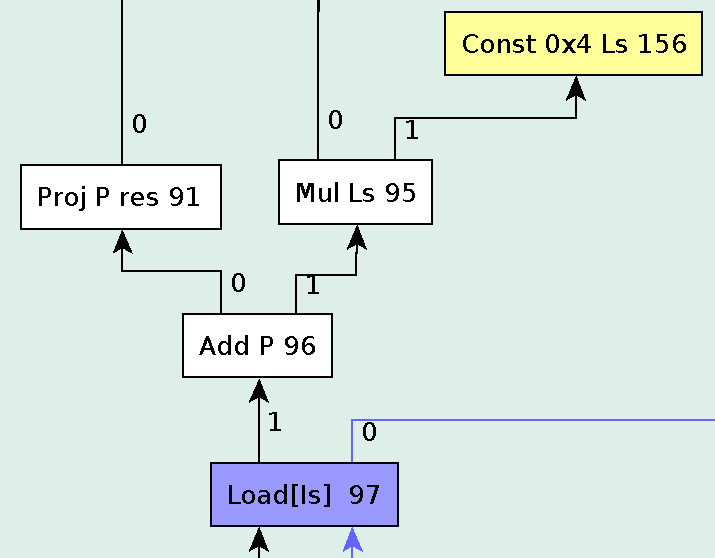
\includegraphics[scale=0.3]{images/instruction-selection.png}
			\end{figure}
		\end{column}
	\end{columns}
\end{frame}

\begin{frame}{Instruction Selection - Tree/DAG Matching}
	\begin{columns}
		\begin{column}{0.5\textwidth}
			\begin{itemize}
				\item Each target instruction is represented as an IR pattern
				\item BUPM finds optimal pattern for each node
				\item Optimal DAG Matching is in general NP-Complete
				\vspace{2em}
				\item \texttt{v3 <- load [V2 + V1 * 0x4]}
			\end{itemize}
		\end{column}

		\begin{column}{0.5\textwidth}
			\begin{figure}
				\centering
				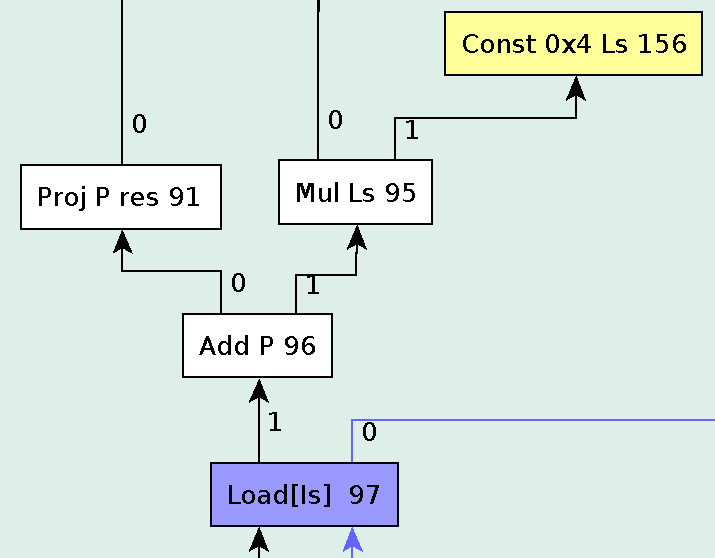
\includegraphics[scale=0.3]{images/instruction-selection.png}
			\end{figure}
		\end{column}
	\end{columns}
\end{frame}

\begin{frame}{Instruction Selection - Our Approach}
	\begin{columns}
		\begin{column}{0.4\textwidth}
			\begin{itemize}
				\item Greedy tree pattern matching on firm graph
				\item Match on x86 address pattern and fold it into binary instruction
				\item $Const + Base + Index * Scale$
				\vspace{2em}
				\item \texttt{v4 <- add v1 [V2 + V3 * 4]}
			\end{itemize}
		\end{column}
		\begin{column}{0.6\textwidth}
			\vspace{-1em}
			\begin{figure}
				\centering
				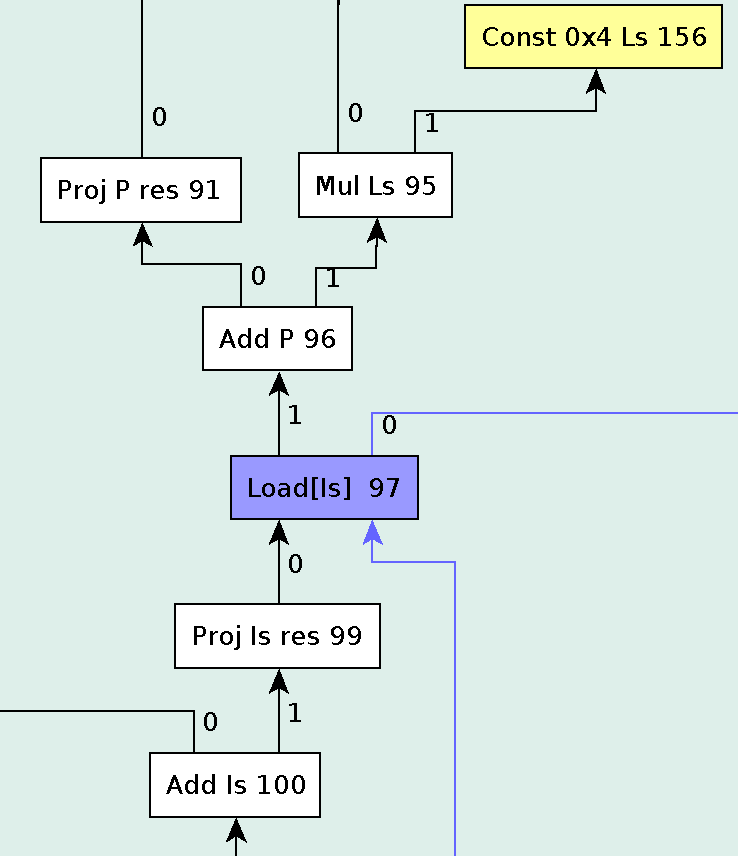
\includegraphics[scale=0.27]{images/memory-match-firm-graph.png}
			\end{figure}
		\end{column}
	\end{columns}
\end{frame}

\begin{frame}{Our Compiler - Overview}
	\begin{figure}
		\centering
		%\vspace{-10px}
		%\def\scale{0.7}
		\providecommand{\scale}{1}
\usetikzlibrary {positioning,arrows.meta,backgrounds,fit,positioning}
\begin{tikzpicture}[->,node distance=20mm,
	terminal/.style={
	% The shape:
	rectangle,minimum size=6mm,rounded corners=3mm,
	% The rest
	draw=black,
	font=\ttfamily},
	el/.style={
		midway,
		above,
	}]

	\node (input) [terminal] {Input};
	\node (ast) [terminal,right=of input] {AST};
	\node (firm) [terminal,right=of ast] {\textsc{Firm}};
	\node (llir) [terminal,below=of ast] {LLIR};
	\node (sir) [terminal,below=of firm] {SIR};
	\node (asm) [terminal,right=of sir] {Assembly};

\draw
	(input)	edge [el] node [] {} (ast)
	(ast)	edge [el] node [] {} (firm)
	(firm)	edge [el,out=-90,in=90] node [right] {instruction selection} (llir)
	(llir)	edge [el] node [] {scheduling} (sir)
	(sir)	edge [el,loop below] node [] {register allocation} (sir)
			edge [el] node [] {} (asm);


\begin{scope}[on background layer]
\node [fill=black!10,inner sep=20,fit=(ast) (firm)] {};
\node [fill=black!10,inner sep=26,fit=(llir) (sir)] {};
\end{scope}

% \draw [->] (input) 
% 		-- (ast) node [el] {}
% 		-- (firm) node [el] {}
% 		-- (llir) [loop,below]
% 		-- (llir) node [el,right] {instruction selection}
% 		-- (sir) node [el] {scheduling}
% 		-- (asm) node [el] {};
\end{tikzpicture}
\def\scale{1}

	\end{figure}
\end{frame}

\begin{frame}{Frontend}
	\begin{itemize}
		\item Parser recovery (with extra error productions)
		\item Rust-style error messages
	\end{itemize}

	\begin{figure}
		\centering
		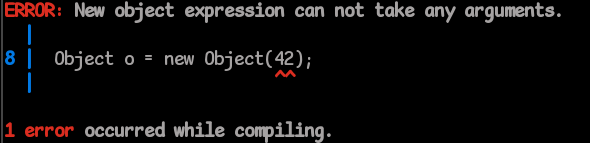
\includegraphics{images/error_message.png}
	\end{figure}
\end{frame}

\begin{frame}{Middleend}
	\begin{columns}
		\begin{column}{0.4\linewidth}
			\begin{itemize}
				\item Sparse Conditional Constant Propagation
				\item Misc. arithmetic simplifications
				\item Loop Invariant Code Motion
				\item Common Subexpression Elimination
				\item Function inlining
				\item Load/Store optimization
			\end{itemize}%
		\end{column}

		\begin{column}{0.25\linewidth}
			\vspace{-3em}
			\begin{figure}
				\centering
				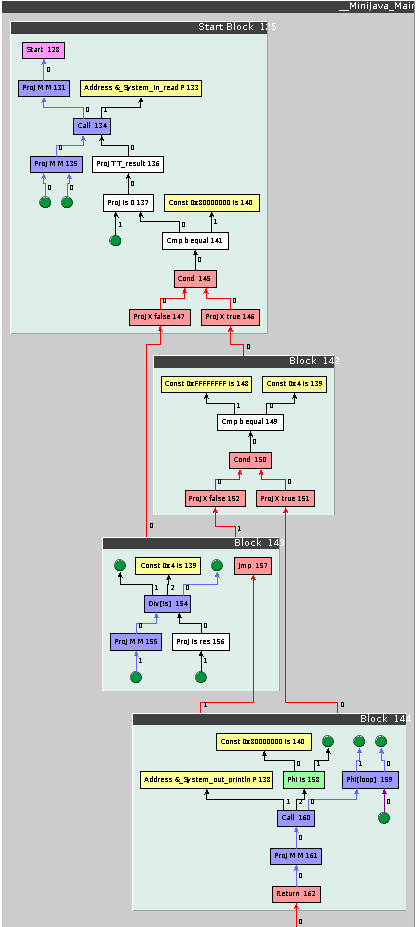
\includegraphics[scale=0.3]{images/optimization-before.png}
			\end{figure}
		\end{column}

		\begin{column}{0.3\linewidth}
			\begin{figure}
				\centering
				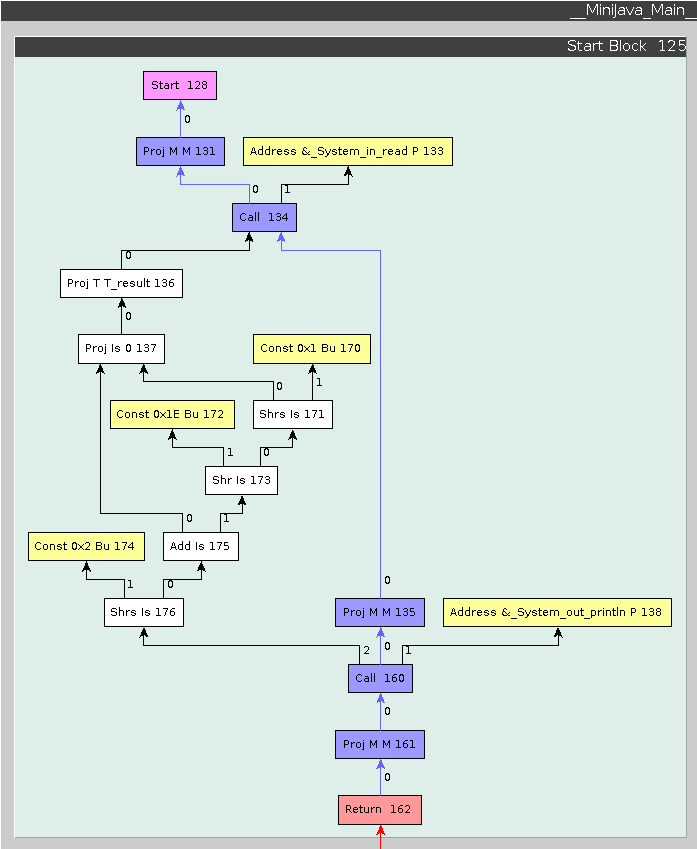
\includegraphics[scale=0.2]{images/optimization-after.png}
			\end{figure}
		\end{column}
	\end{columns}
\end{frame}

\begin{frame}{Backend - LLIR}
	\framesubtitle{Low-Level Intermediate Representation}
	
	\begin{columns}
		\begin{column}{0.35\textwidth}
			\begin{itemize}
				\item Preserves firm dependencies
				\item Not in SSA
				\item Nodes represent x86 instructions
			\end{itemize}
		\end{column}

		\begin{column}{0.65\textwidth}
			\vspace{-3em}
			\begin{figure}
				\centering
				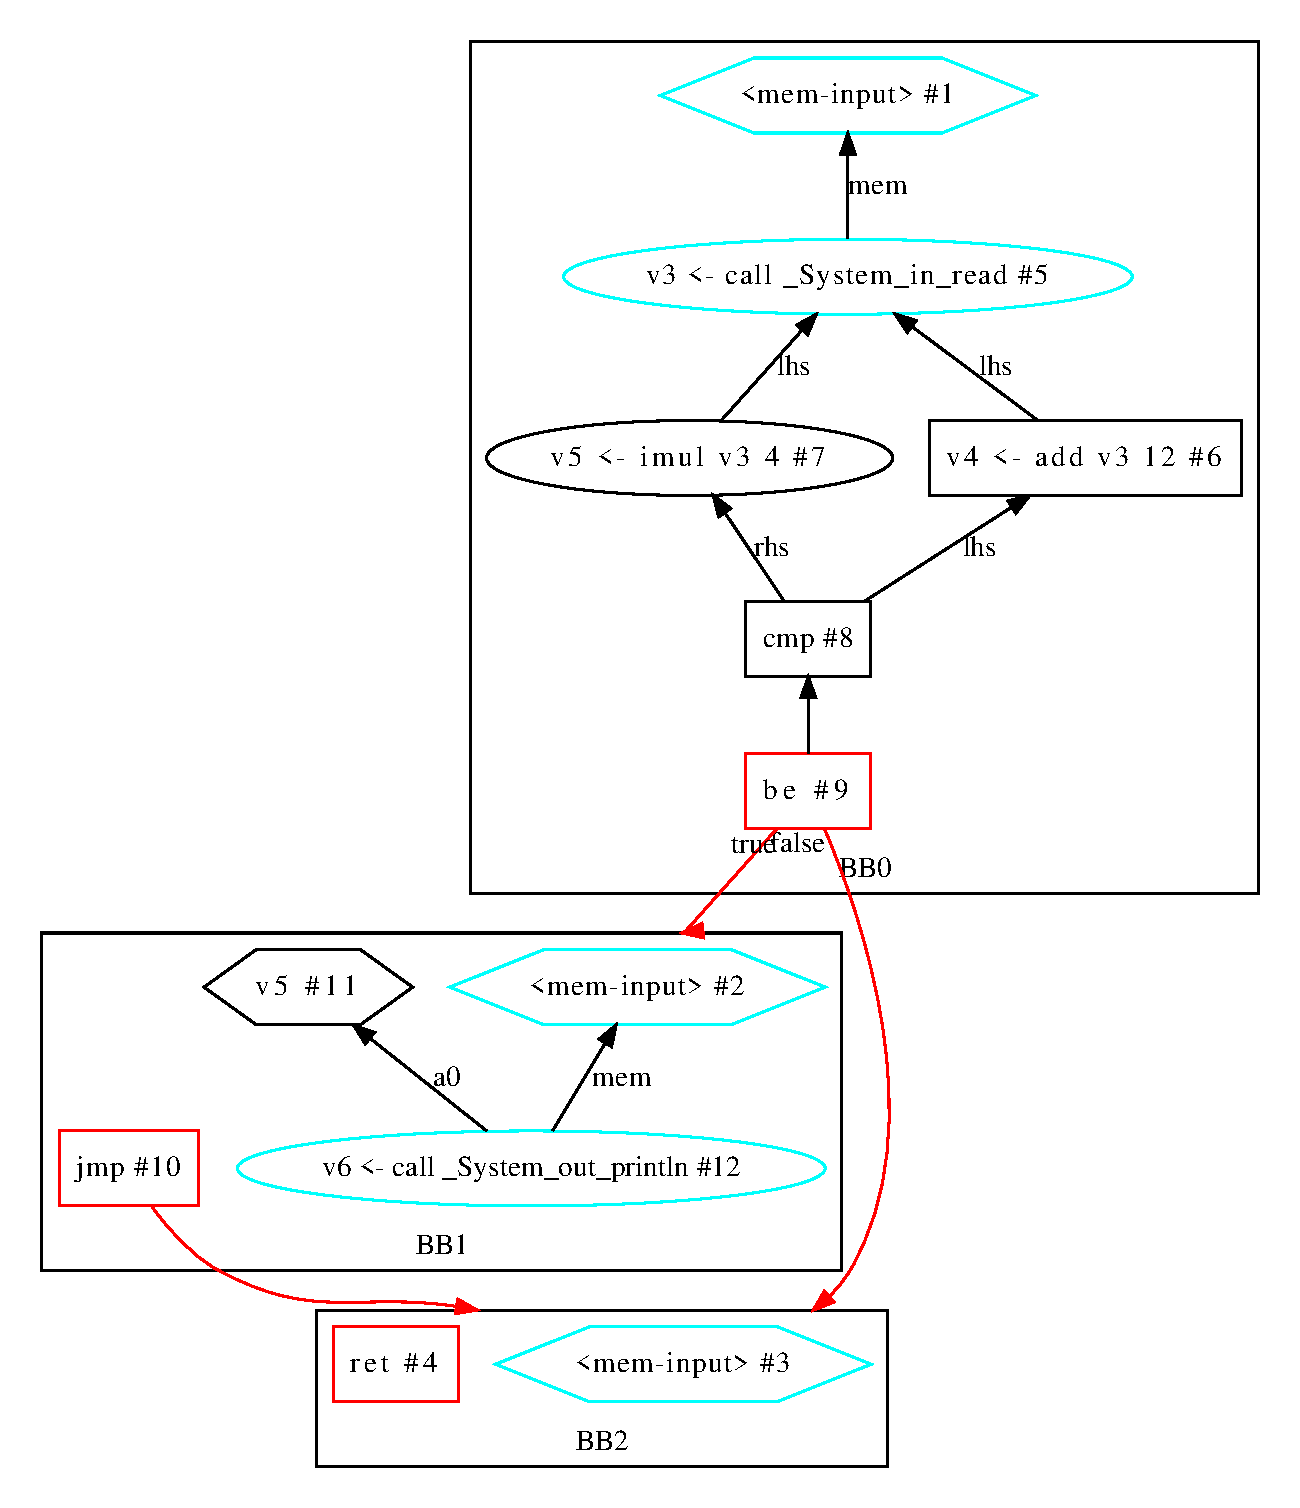
\includegraphics[scale=0.26]{images/llir-example}
			\end{figure}
		\end{column}
	\end{columns}
\end{frame}

\begin{frame}{Backend - SIR}
	\framesubtitle{Scheduled Intermediate Representation}
	
	\begin{columns}
		\begin{column}{0.5\textwidth}
			\begin{itemize}
				\item Includes scheduling information
				\item Easier for register allocation
			\end{itemize}
		\end{column}
	
		\begin{column}{0.5\textwidth}
			\begin{figure}
				\centering
				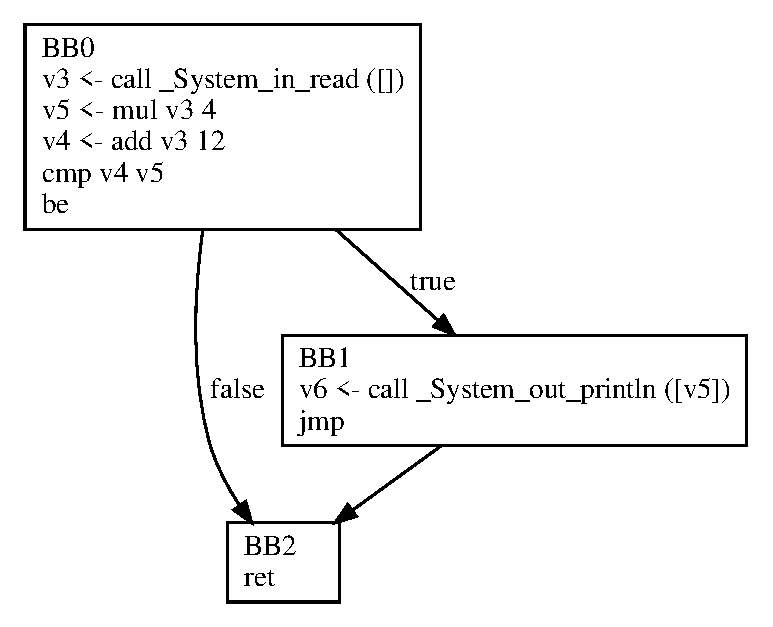
\includegraphics[scale=0.6]{images/sir-before-reg-alloc}
			\end{figure}
		\end{column}
	\end{columns}
	
\end{frame}

\begin{frame}{Backend - SIR}
	\framesubtitle{Scheduled Intermediate Representation}
	
	\begin{columns}
		\begin{column}{0.5\textwidth}
			\begin{itemize}
				\item Our own global register allocator algorithm
				\item Peephole optimizer
			\end{itemize}
		\end{column}

		\begin{column}{0.5\textwidth}
			\begin{figure}
				\centering
				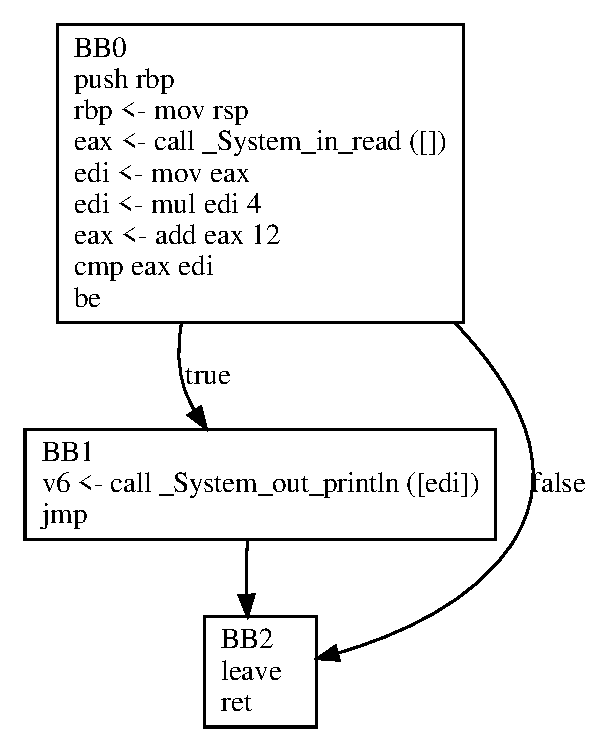
\includegraphics[scale=0.5]{images/sir-after-reg-alloc}
			\end{figure}
		\end{column}
	\end{columns}
\end{frame}

\begin{frame}{Compiler - Gruppe 5}
	\vspace{-3em}
	\begin{columns}
		\begin{column}{0.3\textwidth}
			\begin{itemize}
				\item 21337 LOC
				\item 402 commits
			\end{itemize}
		\end{column}

		\begin{column}{0.5\textwidth}
			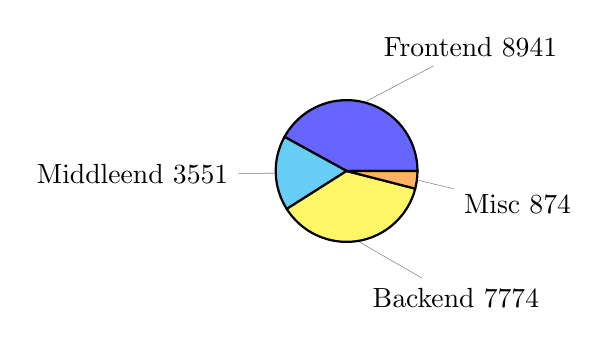
\begin{tikzpicture}[scale=0.3]
				\pie[hide number, text=pin]{42/{Frontend 8941}, 17/Middleend 3551, 37/Backend 7774, 4/Misc 874}
			\end{tikzpicture}
		\end{column}
	\end{columns}

	\begin{figure}
		\centering
		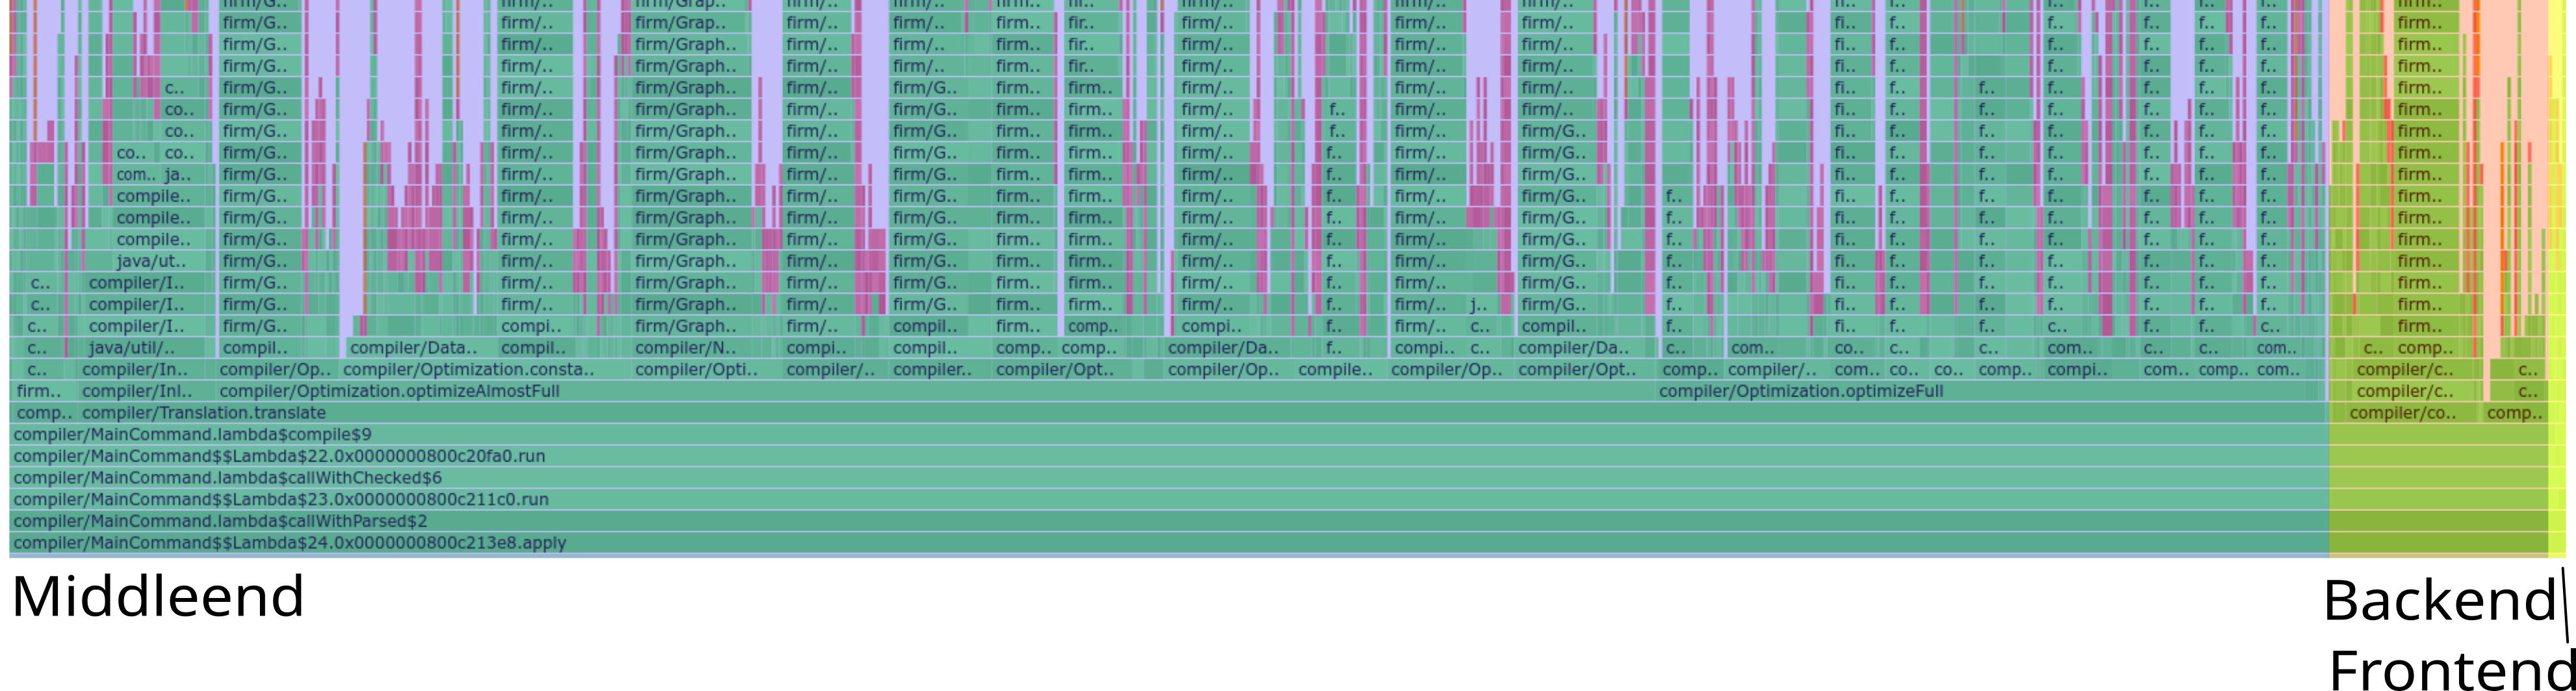
\includegraphics[scale=0.3]{images/flamegraph_annotated}
	\end{figure}
\end{frame}

%\appendix
%\beginbackup

%\begin{frame}{References}
%\printbibliography
%\end{frame}

%\backupend

\end{document}
